\documentclass[a4paper]{article}

\usepackage[utf8]{inputenc}
\usepackage[T1]{fontenc}
\usepackage{textcomp}
\usepackage[dutch]{babel}
\usepackage{amsmath, amssymb}
\usepackage{hyperref}


% figure support
\usepackage{import}
\usepackage{xifthen}
\pdfminorversion=7
\usepackage{pdfpages}
\usepackage{transparent}
\newcommand{\incfig}[1]{%
  \def\svgwidth{\columnwidth}
  \import{./figures/}{#1.pdf_tex}
}

\pdfsuppresswarningpagegroup=1

\title{Epideemia levik erinevate piirkondade vahel}
\author{Joosep Jääger}

\begin{document}
  \maketitle
  Selle projekti käigus lõin mudeli, mis püüab ennustada, COVID-19 nakatumist
  Eestis, Lätis, Soomes, Venemaal ning maailmas. Mudelis simuleeritakse riigisisest
  nakatumis SEIR mudeli abil. Selles mudelis on neli olekut: vastuvõtlik, kokkupuutunud,
  nakkusohtlik ning taastunud. Iga päeva kohta arvutatakse välja, kui palju igas
  olekus olevate inimeste arv muutub. Valemid on järgmised
  \begin{align}
    S'(t)&=-\beta(t) S(t)(E(t)+I(t))\\
    E'(t)&=\beta(t) S(t)(E(t)+I(t))-\mu E(t)\\
    I'(t)&=E(t)\mu-I(t)\gamma\\
    R'(t)&=I(t)\gamma
  \end{align}
  Simulatsiooni alguses kasutame andmete põhjal saadud nakatunute arve 1. märtsi
  seisuga. Parameetrite leidmiseks katsetasin läbi erinevaid väärtusi kuni graafik
  mudelist saadud graafik kattus piisavalt hästi päris nakatumiste andmetega.
  Katse-eksituse meetodiga sain järgmised parameetrite väärtused:
  \begin{align}
    \beta(t)&=\frac{0.13}{N-1}\phi(t) \\
    \mu&=0.19 \\
    \gamma&=0.09
  \end{align}
  Selleks, et mudelis oleks näha ka aprilli COVID-19 lainet eestis, võtsin kasutusele
  'pandeemiaväsimust' tähistava funktsiooni $\phi(t)$, mille väärtuse arvutamiseks
  kasutan Google Trendsist saadud andmeid otsingusõna "covid-19" kohta. Minu hüpotees on,
  et otsingusõna populaarsus näitab, kui ettevaatlikud inimesed ühel või teisel ajahetkel
  COVID-19 suhtes on ning seega mida populaarsem otsingusõna mingil ajahetkel oli,
  seda aeglasem on sellel ajal COVID-19 levik. Parameetri $\phi(t)$ väärtus on üks sel päeval,
  kui otsingusõna oli kõige populaarsem ning null, kui huvi otsingusõna vastu puudus.
  Selle parameetri kasutamisel on mudelis tõepoolest näha, kuidas Eestis toimub aprillis
  esimene koroonaviiruse laine.
  \begin{figure}
    \centering
    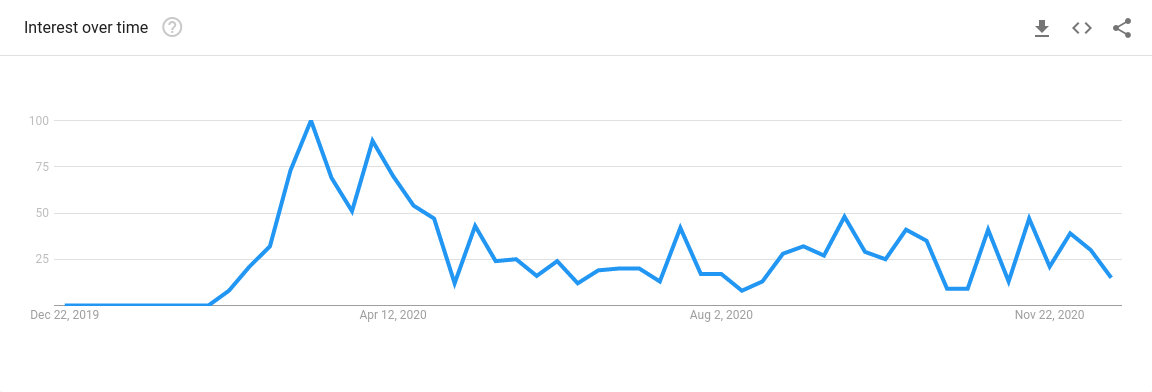
\includegraphics[width=\textwidth]{graphics/trends.png}
    \caption{Otsingusõna "covid-19" populaarsus Eestis. Google Trends.}
  \end{figure}

  Piirkondadevahelise rände simuleerimiseks leidsin vastavate riikide statistikaameti lehelt
  andmed, kui palju on iga teise riigi kohta turiste, kes selles riigis peatuvad.
  Nende andmete põhjal saame moodustada maatriksi, mis näitab, kui palju inimesi rändab
  iga päev meie uuritavate riikide vahel. Kui oleme ühe päeva kohta riigisisest
  SEIR mudelit uuendanud, paigutame vastavalt maatriksi väärtustele inimesi riikide
  vahel ümber. Kahe riigi vahel inimesi liigutades on nende inimeste seas proportsionaalselt
  nii palju nakatunuid, kui on lähteriigis. 

  \begin{figure}
    \centering
    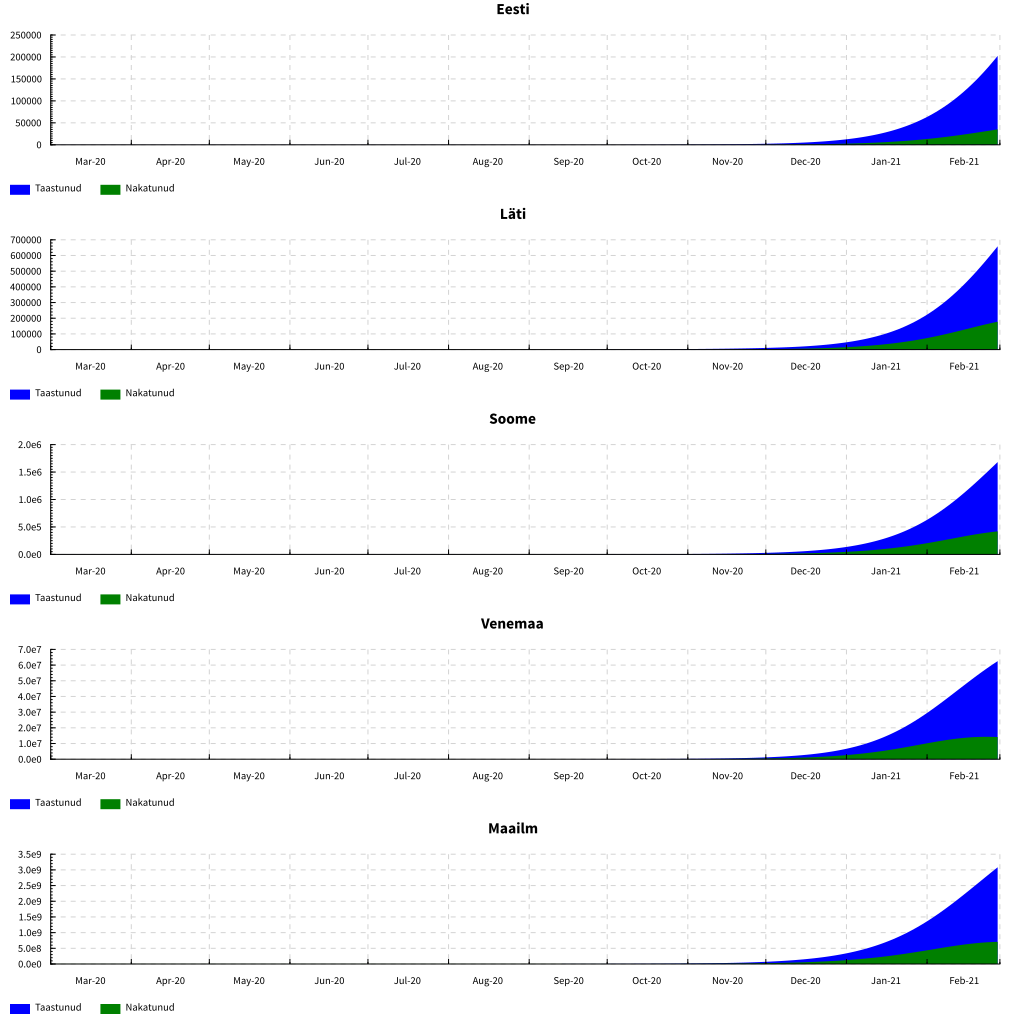
\includegraphics[width=\textwidth]{graphics/year.png}
    \caption{Mudeli ennustus märts 2020 kuni märts 2021.}
  \end{figure}
  \begin{figure}
    \centering
    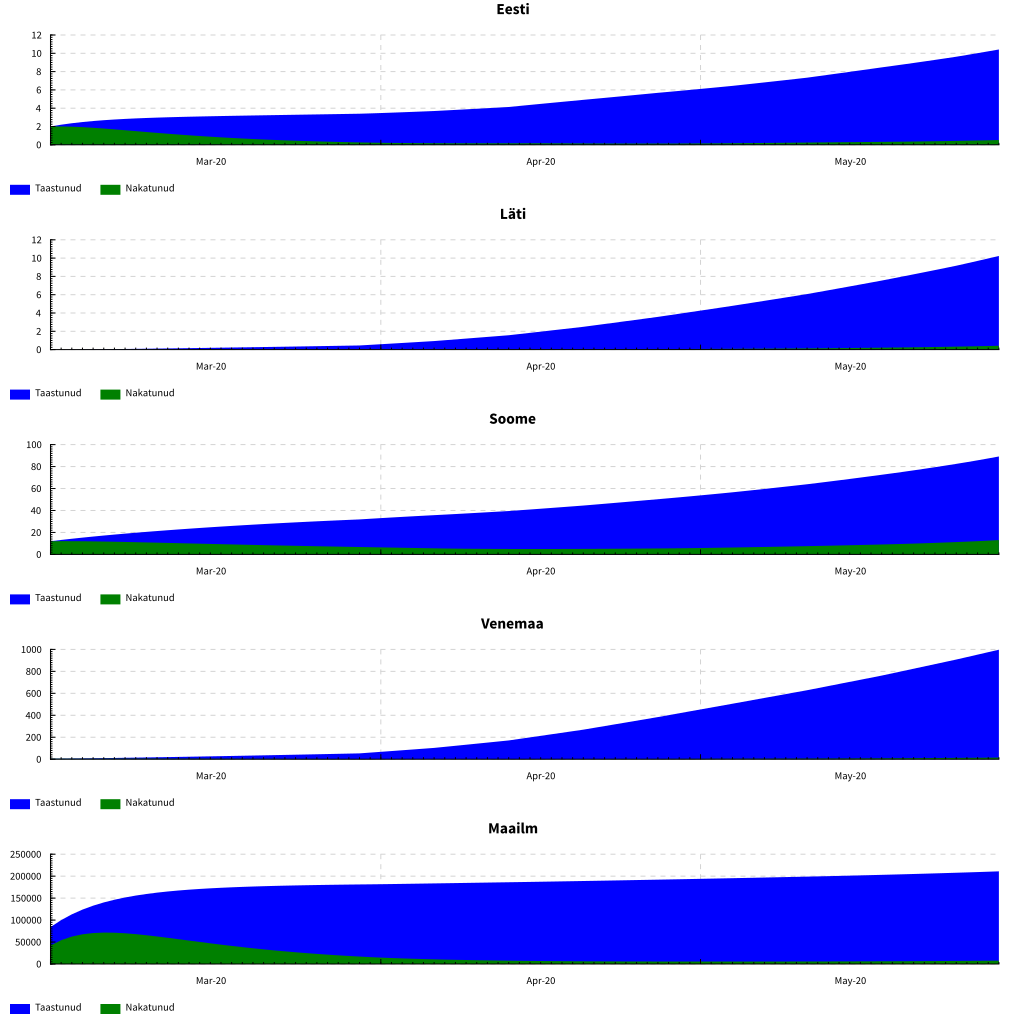
\includegraphics[width=\textwidth]{graphics/twomonths.png}
    \caption{Mudeli ennustus märts 2020 kuni mai 2020.}
  \end{figure}

  \section{Andmete allikad}
  Nakatumiste andmed: \\
  \url{https://www.worldometers.info/coronavirus/} \\
  Eesti turismistatistika: \\
  \url{https://andmed.stat.ee/et/stat/majandus__turism-ja-majutus__majutus/TU14} \\
  Vene turismistatistika: \\
  \url{https://www.ceicdata.com/en/indicator/russia/visitor-arrivals} \\
  Läti turismistatistika: \\
  \url{https://www.ceicdata.com/en/indicator/latvia/visitor-arrivals} \\
  Soome turismistatistika: \\
  \url{https://www.ceicdata.com/datapage/en/indicator/finland/visitor-arrivals} \\
  
\end{document}
